%%This is a very basic article template.
%%There is just one section and two subsections.
\documentclass{article}

\usepackage{amsmath}
\usepackage{amscd}
\usepackage{amssymb}
\usepackage{amsfonts} 
\usepackage{amsthm}
\usepackage{amsfonts}
\usepackage{amsthm}

\usepackage{circuitikz}
\usepackage{pgf}
\usepackage{tikz}
\usetikzlibrary{arrows,snakes,backgrounds}
% \usetikz
\usepackage{subfig}

\usepackage{algpseudocode}
\usepackage{algorithm}

\usepackage[super]{nth}
% \usepackage{appendix}
% \usepackage{listings}
% \usepackage{color}

\usepackage{hyperref}
%\usepackage{url}

\usepackage{cleveref}
\usepackage{cancel}

\usepackage{aviolov_style}
\usepackage{local_style}


\newtheorem{thm}{Theorem}[section]
\newtheorem{lemma}{Theorem}[thm]
% \theoremstyle{definition}
\newtheorem{ex}{Example}[thm]
\newtheorem{defn}{Definition}[thm]

\begin{document}
\begin{figure}[htp] 
\begin{center} 
  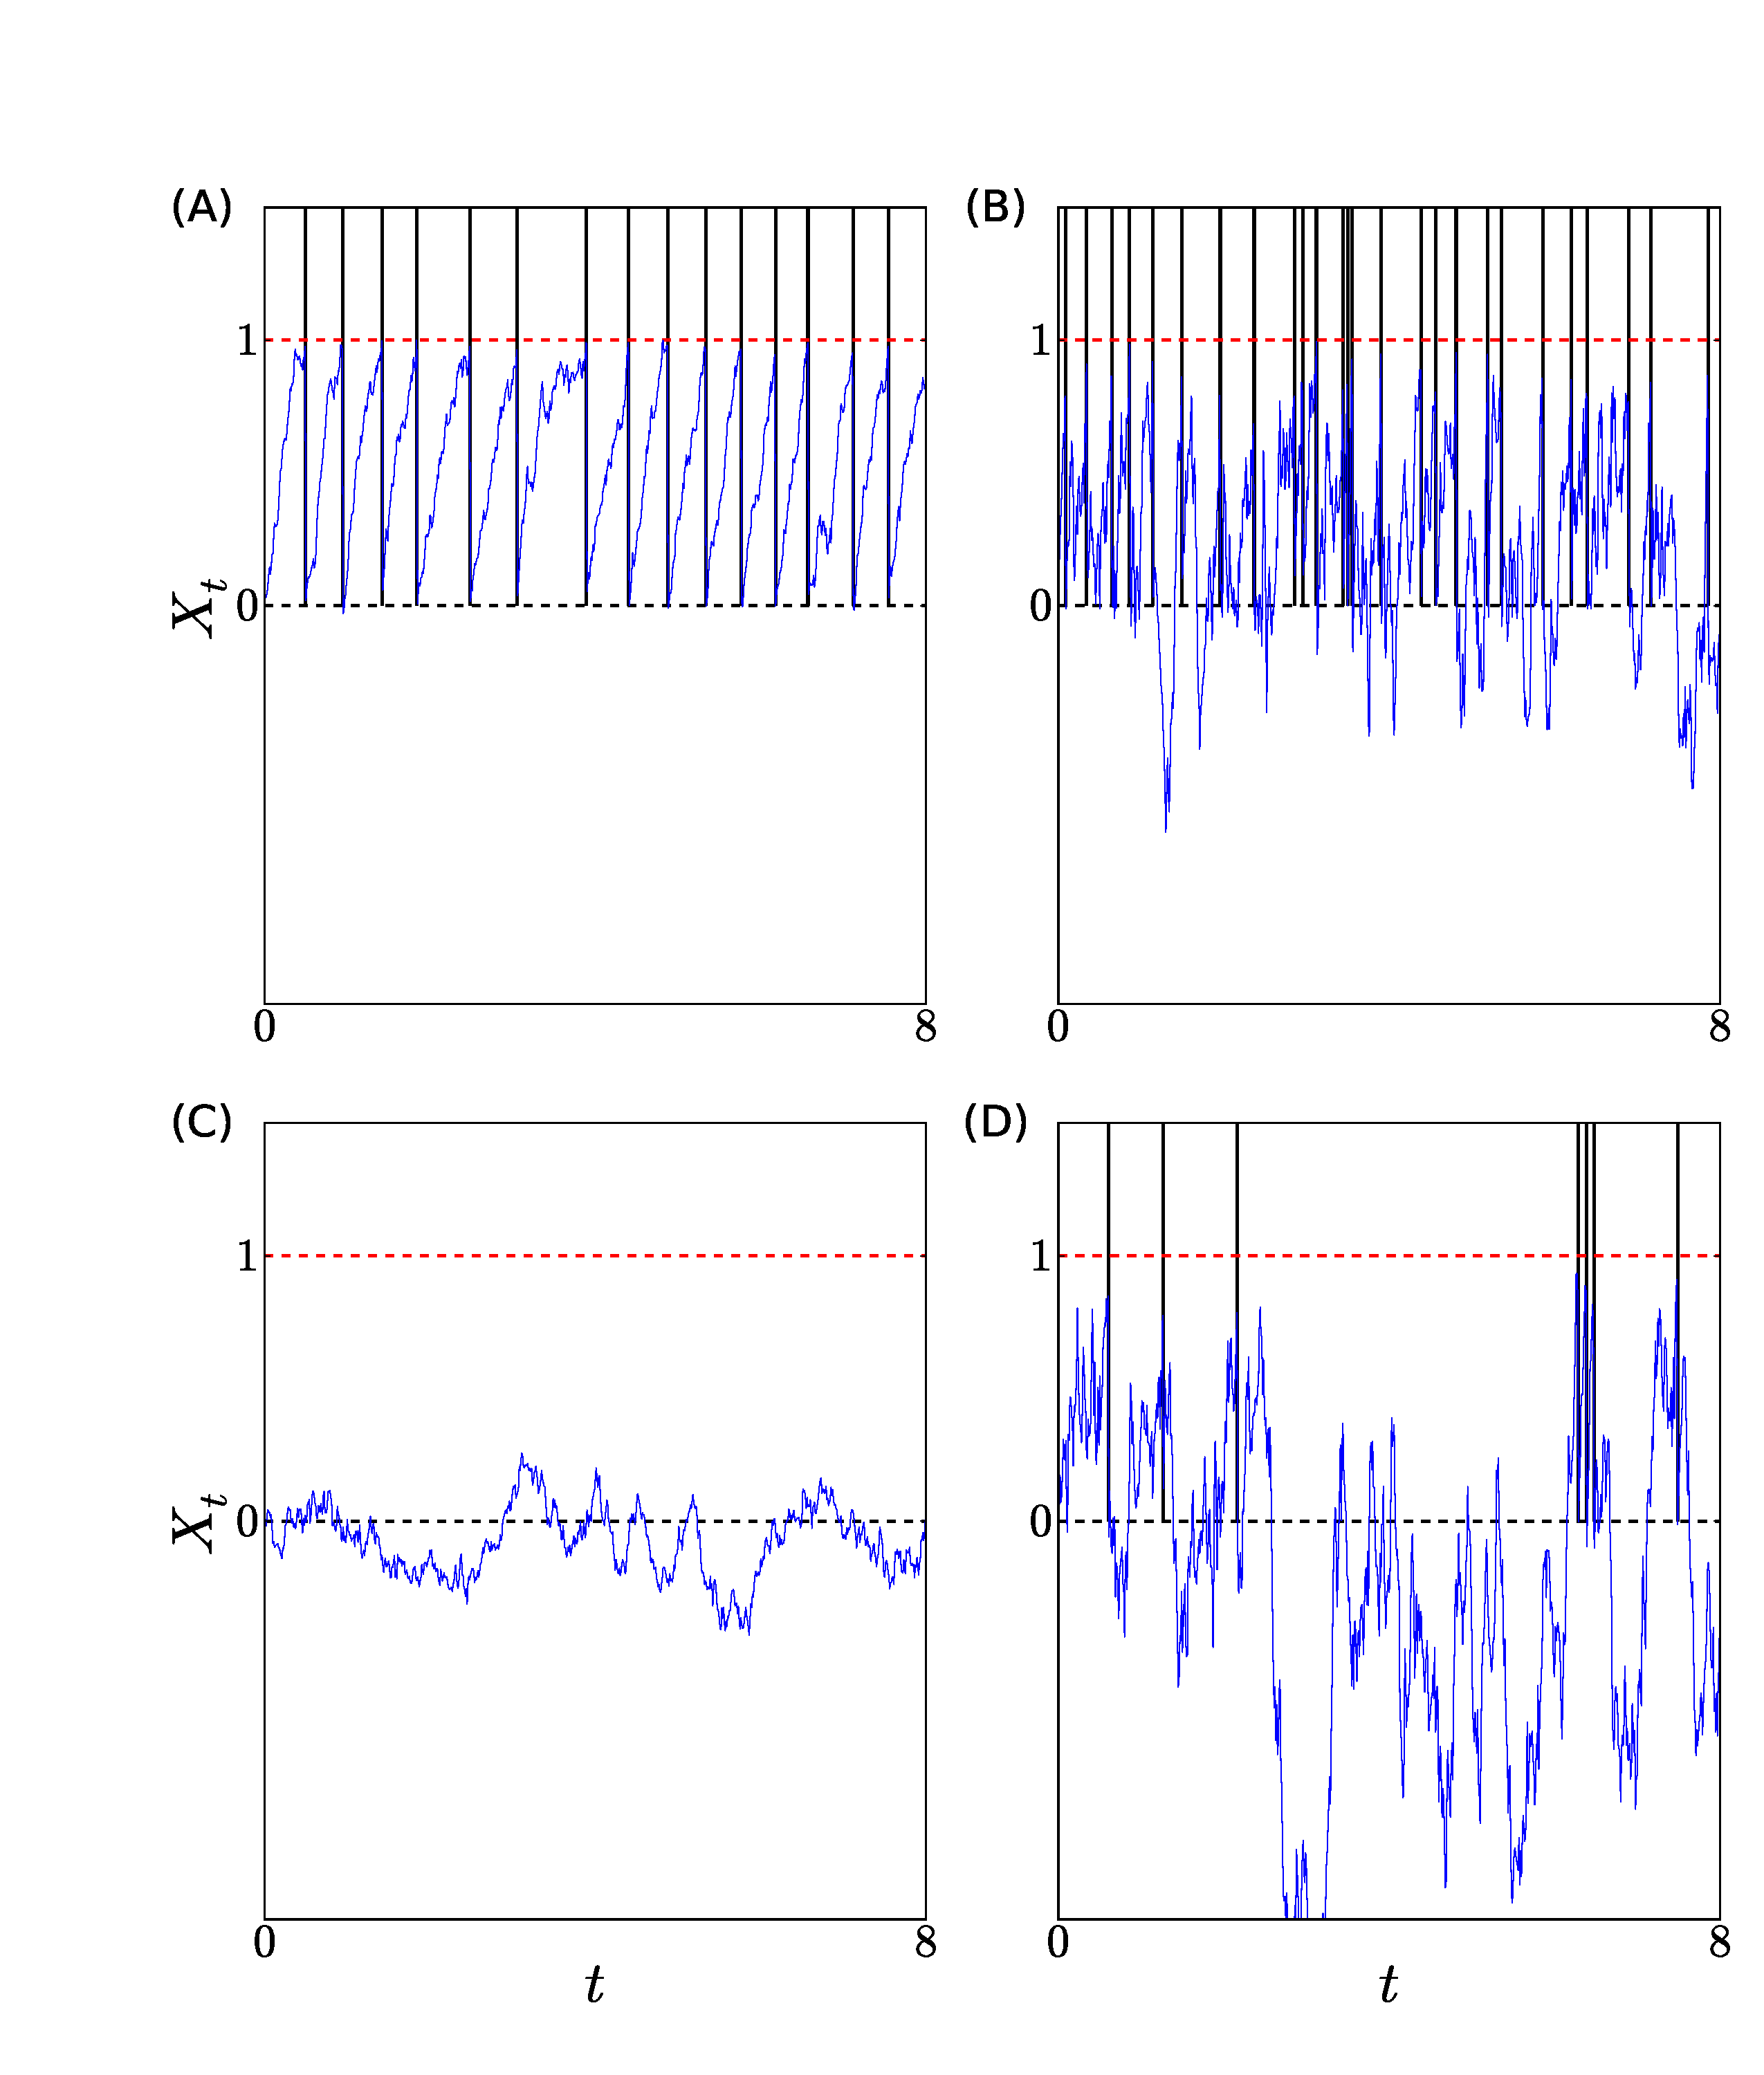
\includegraphics[width=0.99\textwidth]{Figs/PathSimulator/path_T=14_combined.pdf} 
  \caption[labelInTOC]{Example Trajectories from \cref{eq:X_evolution_uo} 
  using the parameter values from \cref{tab:regimes}.  
  A) Supra-Threshold-Low-Noise  
  B) Supra-Threshold-High-Noise  
  C) Sub-Threshold-Low-Noise 
  D) Sub-Threshold-High-Noise.  
  Note the multiple crossings very close together in the high-noise regimes 
  in B and D. } 
  \label{fig:regime_path_examples} 
\end{center} 
\end{figure} 
\begin{figure}[htp] 
\begin{center} 
  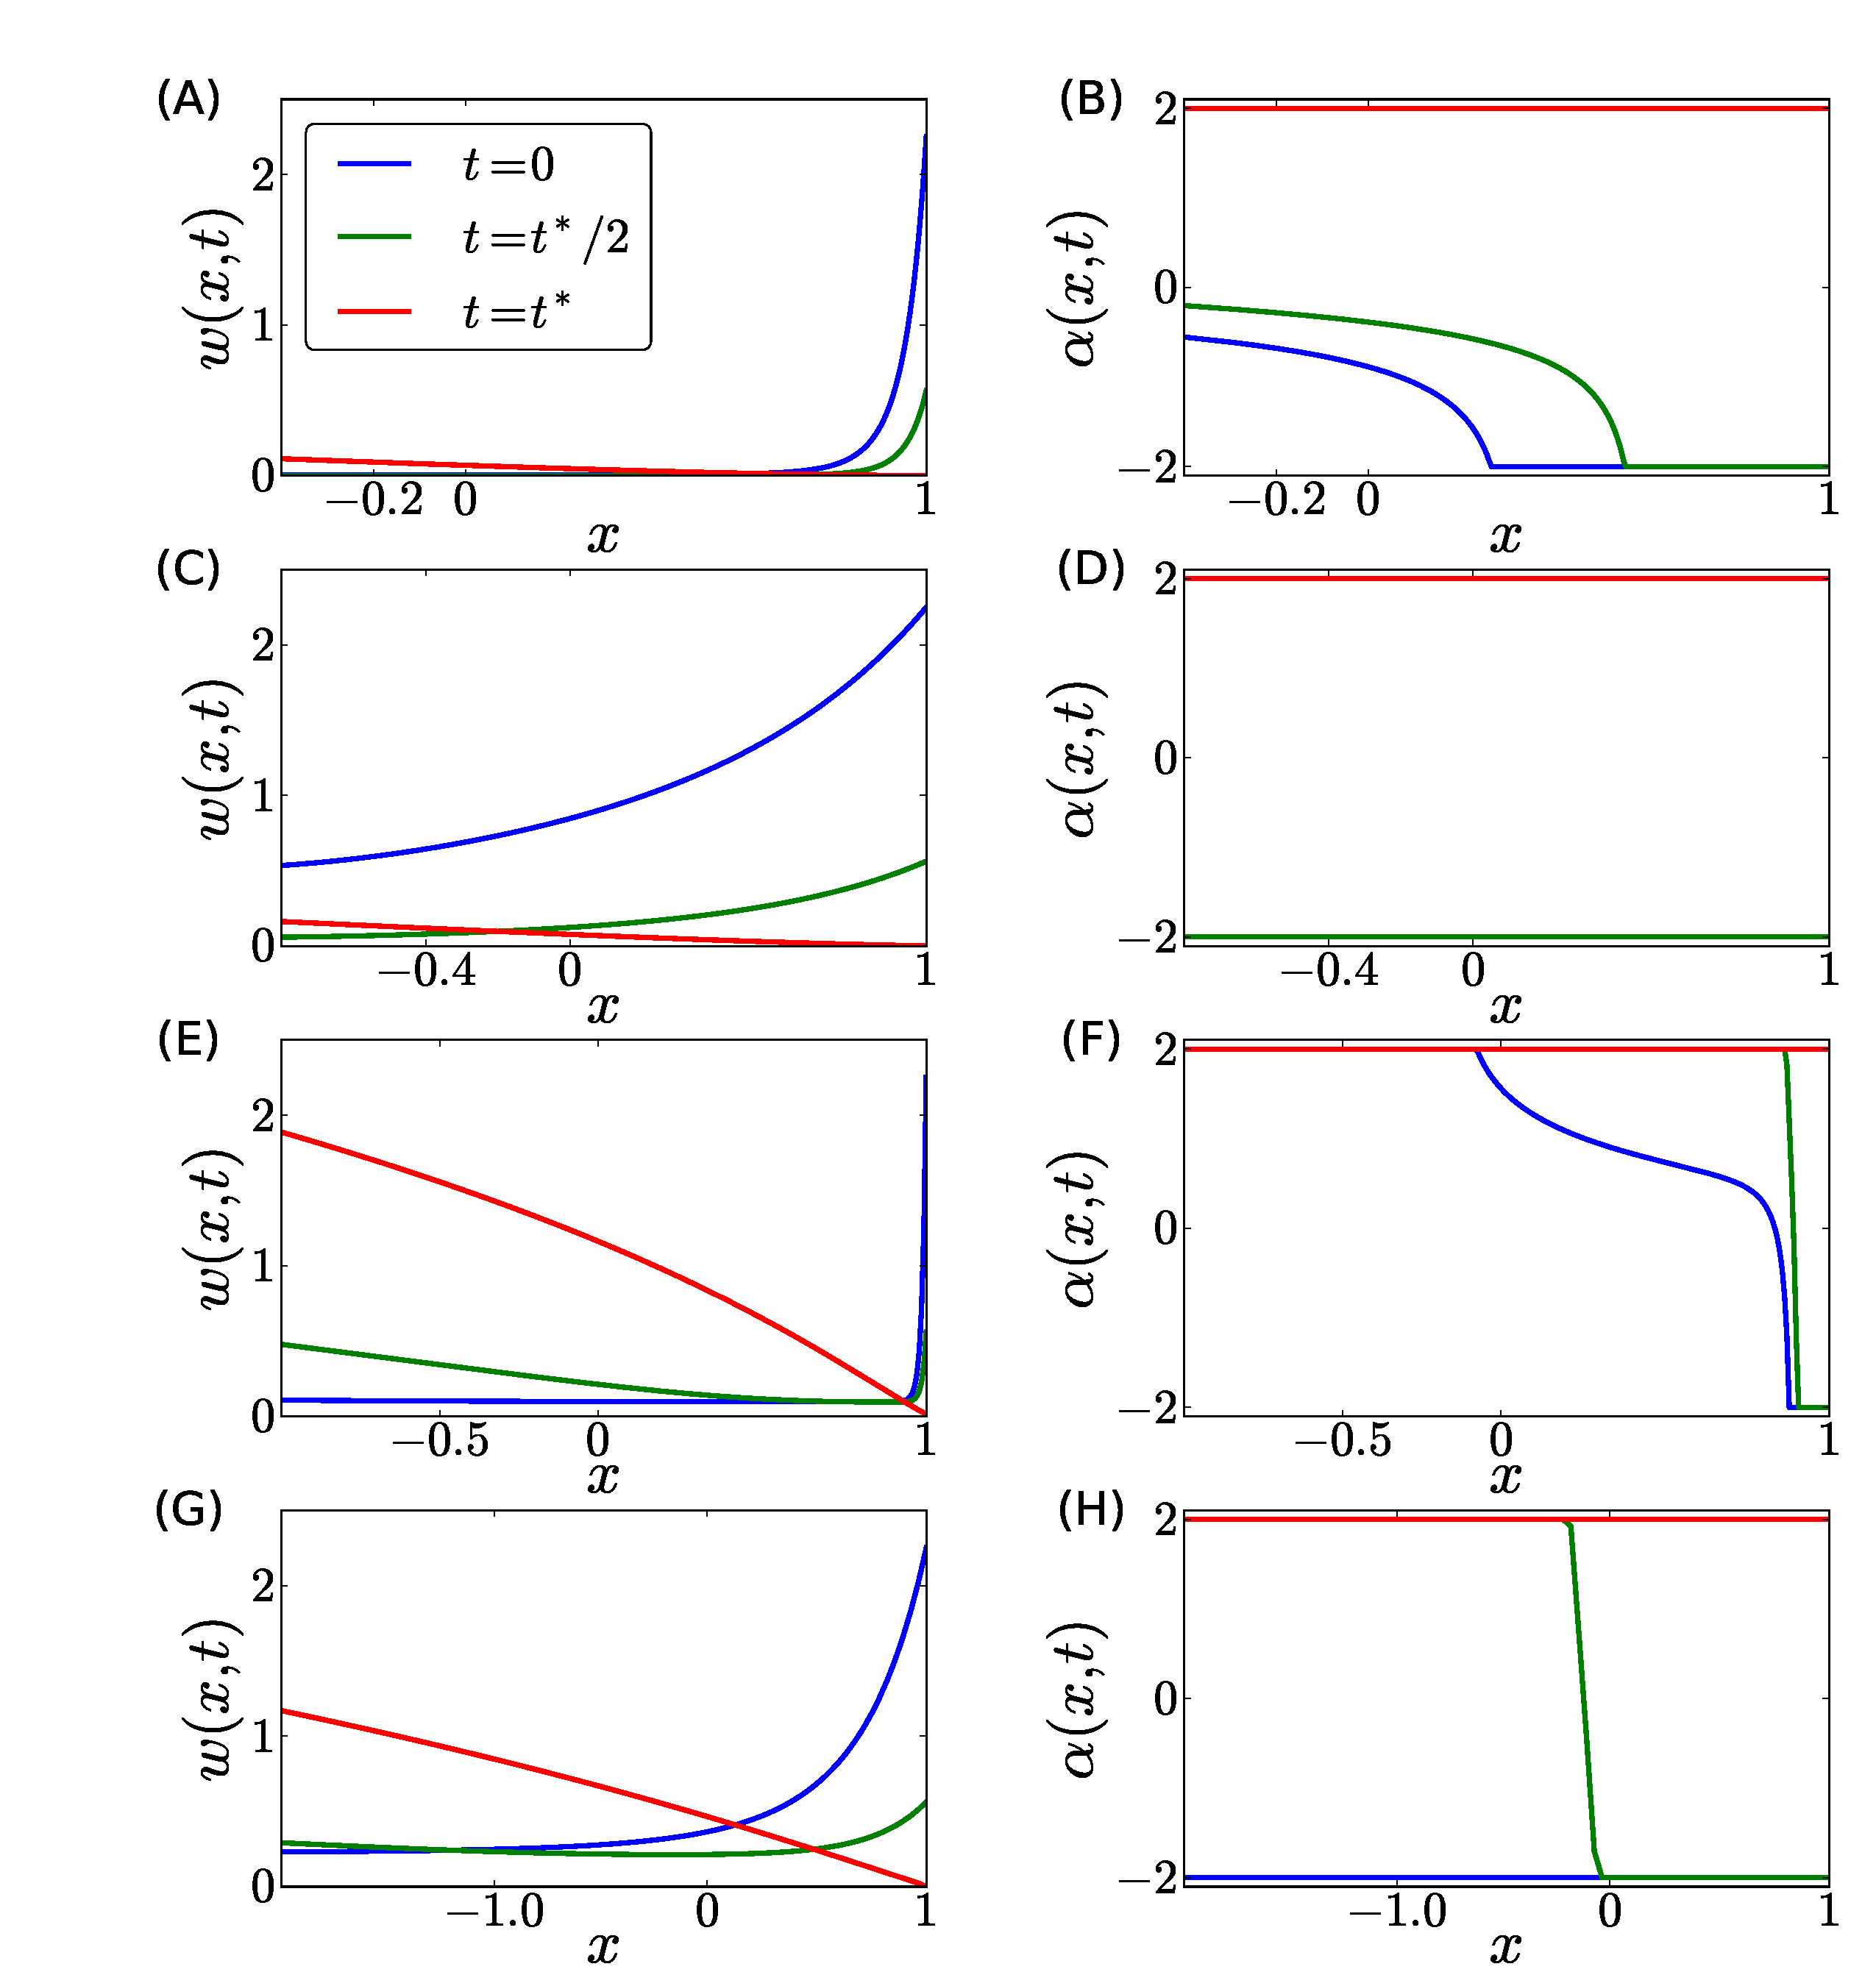
\includegraphics[width=\textwidth]{Figs/HJB/Regimes_vc_cuts.pdf} 
  \caption[labelInTOC]{Snapshots of the value function, $\v$, on the left and on 
  the optimal control, $\a$, on the right for $t$ fixed, at the start (blue), 
  mid-point (green) and end-point (red), for each of the four regimes. 
  The desired spike time is set to $\T=1.5$ assuming the previous spike was at 
  $t=0$, the energy penalty, $\eps = 0.001$. The control bounds are $\a \in 
  [-2,2]$.  
  Note that all red value function curves go to zero at the threshold to satisfy 
  the upper BC in \cref{eq:OC_LS_HJB_full}. 
  Note that the green and blue 
  curves in F) are lying on top of each other for all $x$. 
  \\ 
  A,B) Supra-Threshold-Low-Noise 
  C,D) Supra-Threshold-High-Noise 
  E,F) Sub-Threshold-Low-Noise 
  G,H) Sub-Threshold-High-Noise 
  } 
\label{fig:HJB_4regimes_value_control_cuts} 
\end{center} 
\end{figure} 
\begin{figure}[h!] 
\begin{center} 
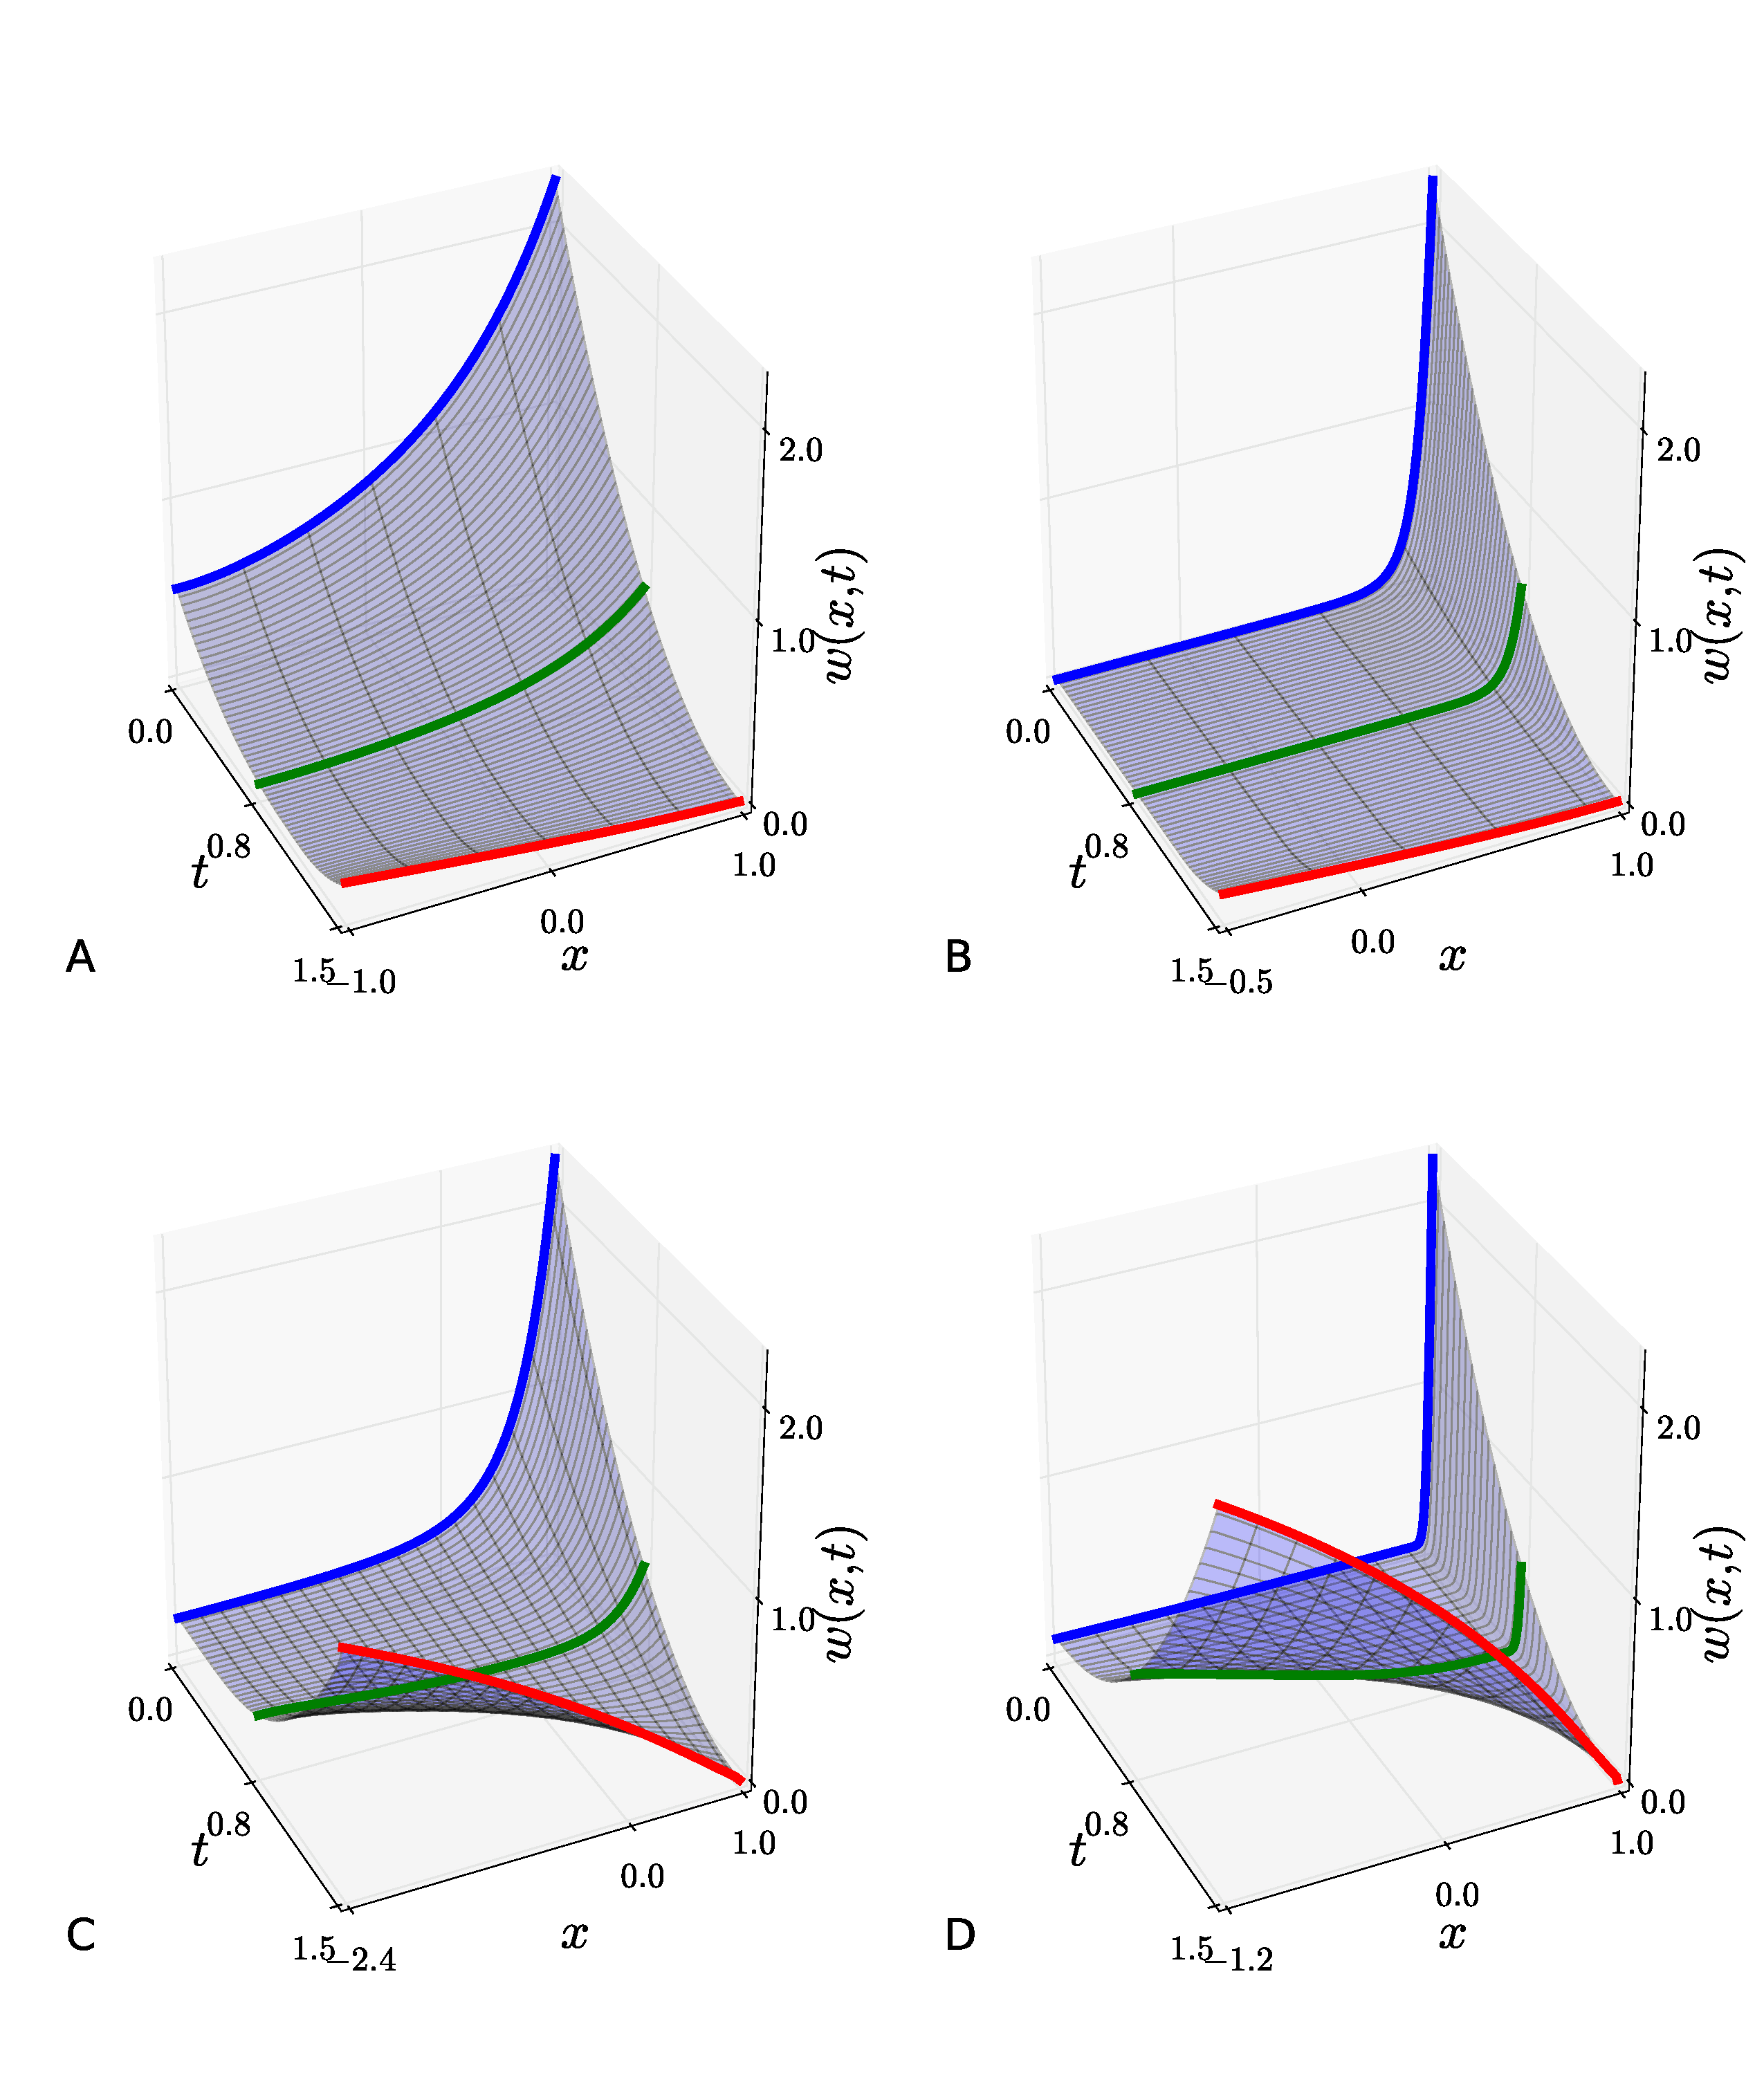
\includegraphics[width=0.99\textwidth]{Figs/HJB/Regimes_valuesurf.pdf} 
\caption{The numerical solution for the value function $\v(x,t)$ HJB PDE, 
\cref{eq:OC_LS_HJB_full}, for the four different parameter regimes. 
The desired spike time is set to $\T=1.5$. 
The control bounds are $\a \in [-2,2]$.  
The coloured contours for fixed $t$ plotted in thick correspond to the 
curves plotted in the left panels of \cref{fig:HJB_4regimes_value_control_cuts} 
(blue: $t=0$, green: $t=t*/2$, red: $t=t*$). 
\\ 
A) Supra-Threshold-Low-Noise 
B) Supra-Threshold-High-Noise 
C) Sub-Threshold-Low-Noise  
D) Sub-Threshold-High-Noise  } 
\label{fig:HJB_4regimes_value_surf} 
\end{center} 
\end{figure} 
\begin{figure}[htp] 
\begin{center} 
  \includegraphics[width=\textwidth]{Figs/FP_Adjoint/Regimes_cs_singleplot.pdf} 
  \caption[labelInTOC]{The deterministic optimal controls for each parameter 
  regime as functions of time, $t \in [0, \T]$. 
  The desired spike time is set to $\T=1.5$, the energy penalty, $\eps 
  = 0.001$ and the bounds are $\a \in [-2,2]$. 
  From left-to-right, the control curves correspond to the 
  Sub-Threshold-Low-Noise, Sub-Threshold-High-Noise, Super-Threshold-High-Noise, 
  Sub-Threshold-Low-Noise regimes 
  } 
  \label{fig:FBK_Regimes_cs} 
\end{center}   
\end{figure}    
\begin{figure}[h]   
\begin{center} 
\subfloat[Supra-Threshold Low-Noise]{ 
  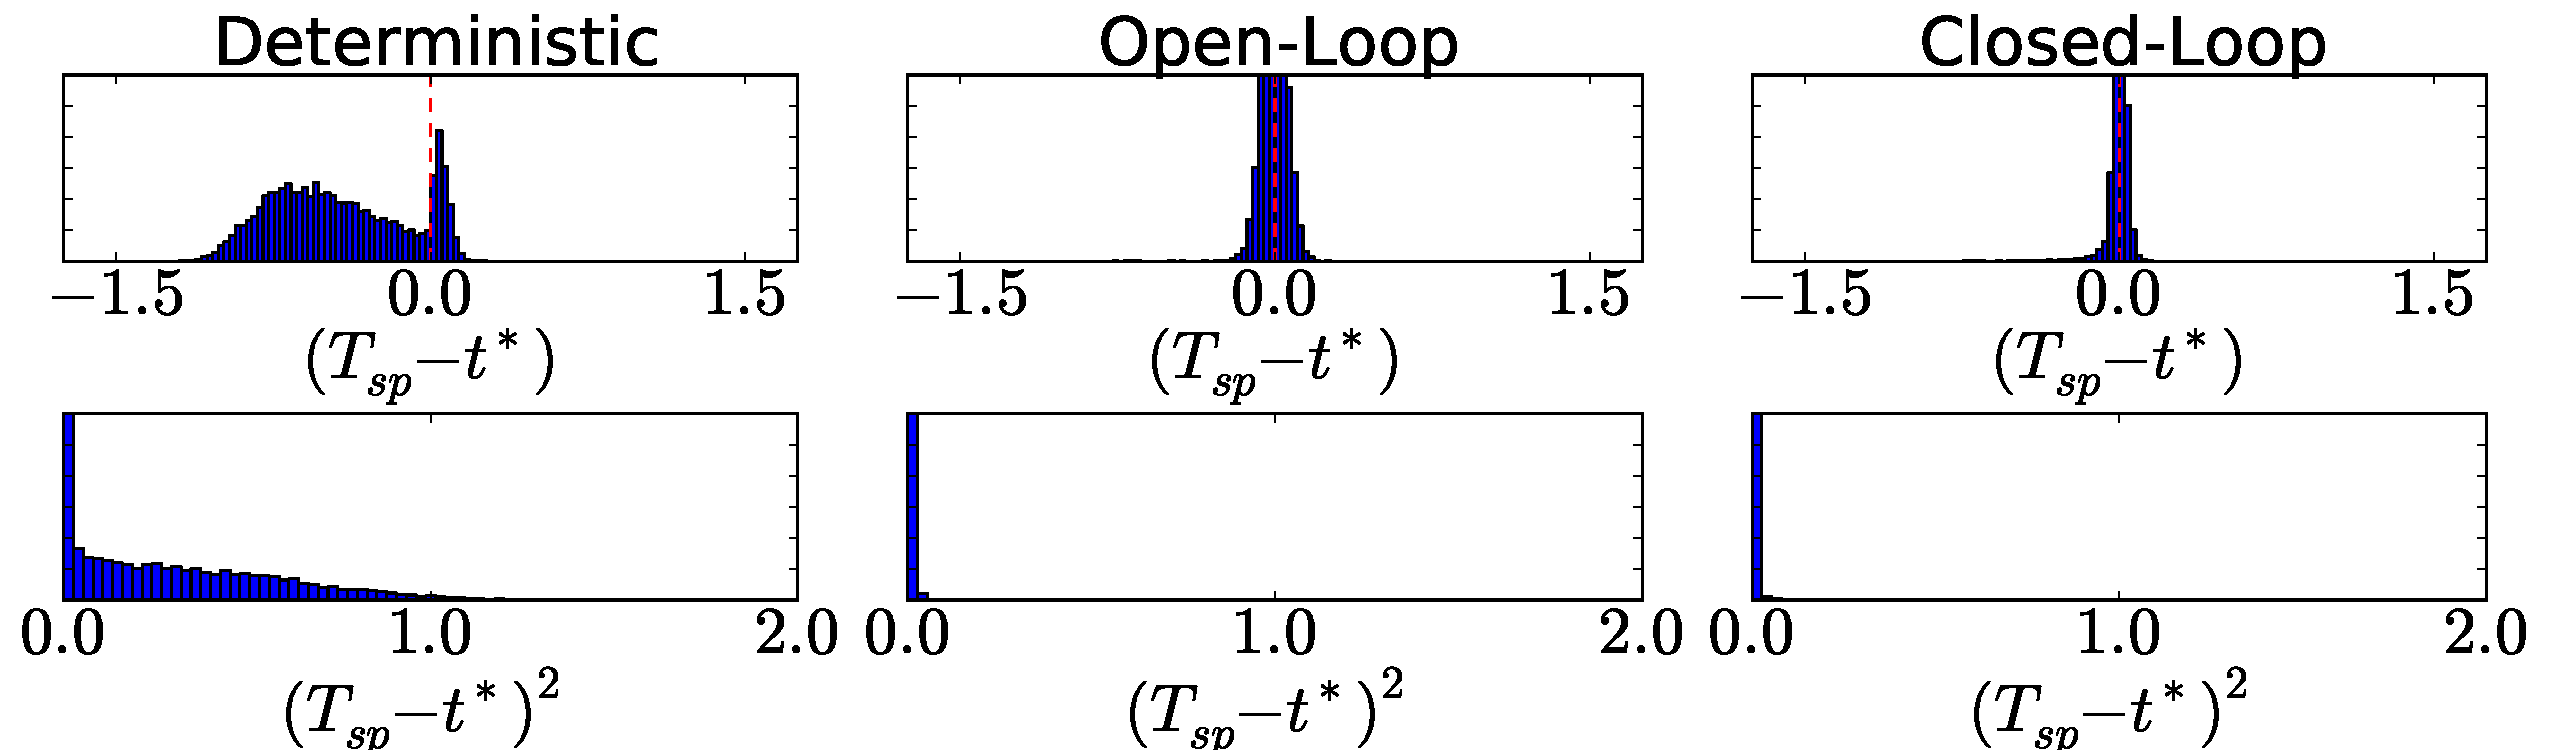
\includegraphics[width=\textwidth] 
  {Figs/ControlSimulator/Regimes_SUPT_ln_errors_hist.pdf} 
} 
\\ 
\subfloat[Supra-Threshold High-Noise]{ 
  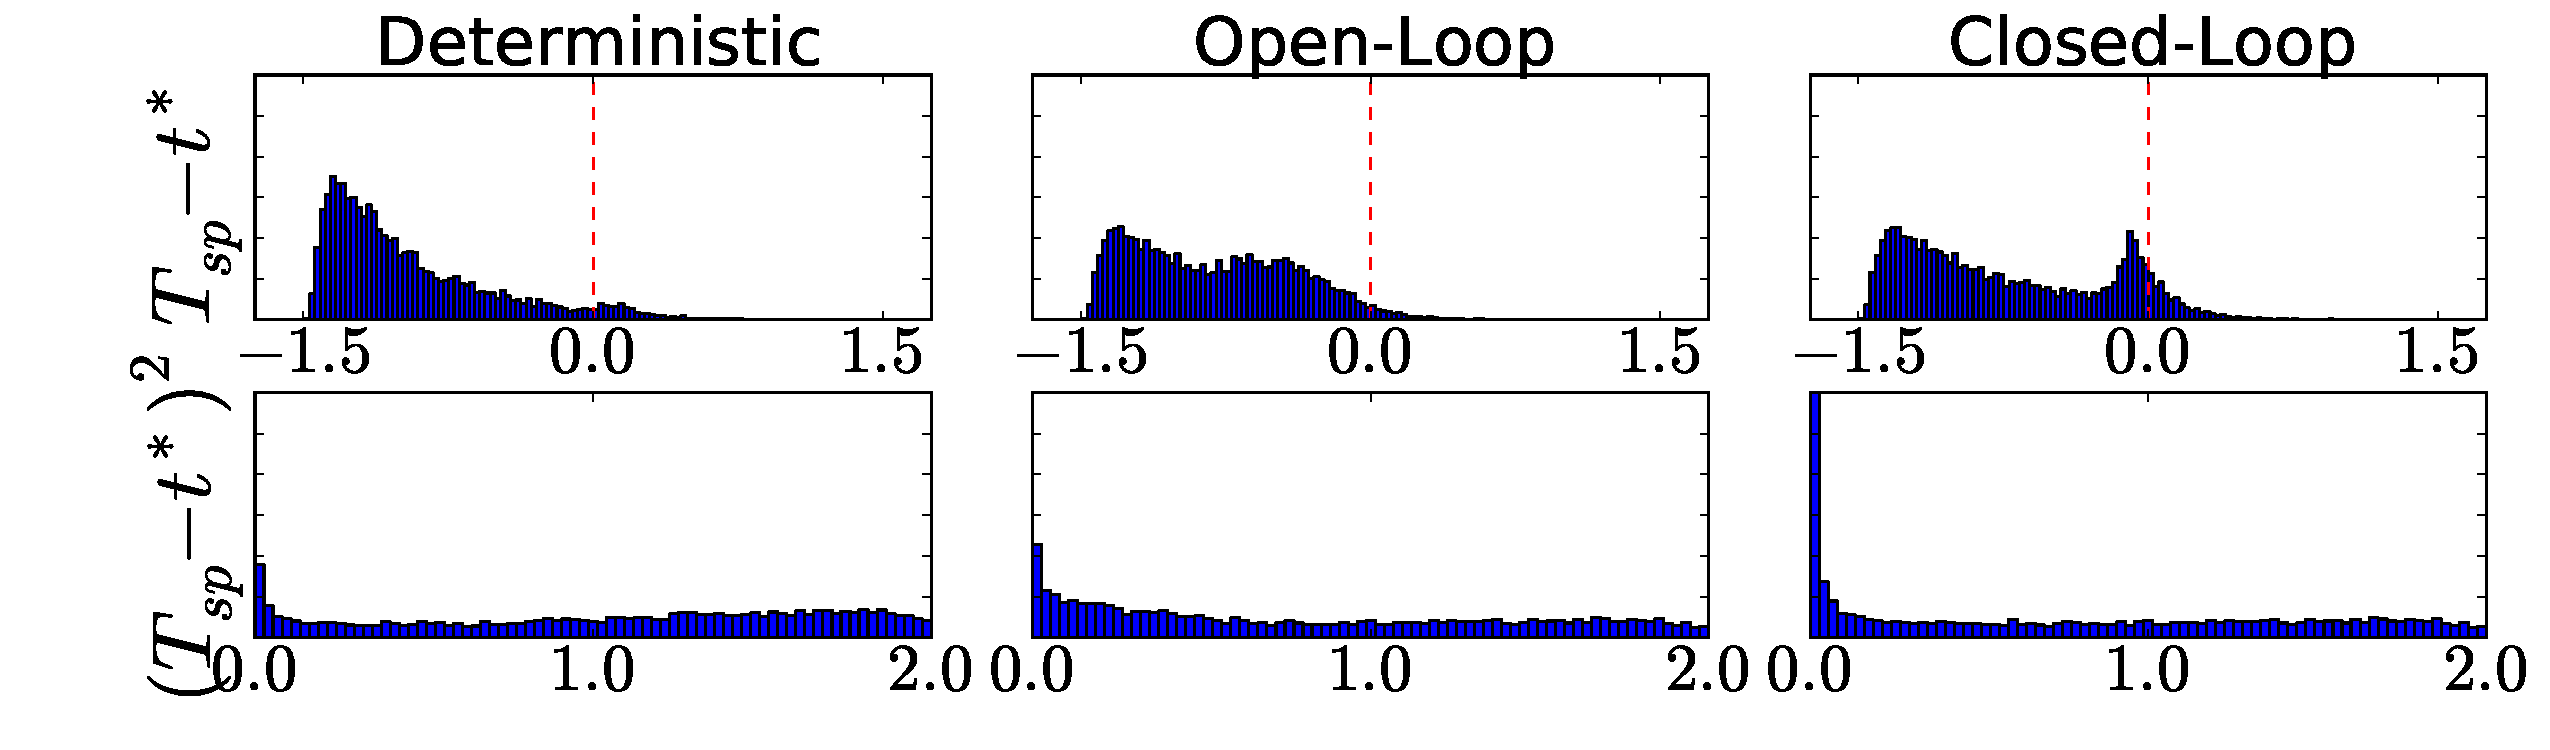
\includegraphics[width=\textwidth] 
  {Figs/ControlSimulator/Regimes_SUPT_HN_errors_hist.pdf} 
  } 
  \\ 
\subfloat[Sub-Threshold Low-Noise]{ 
  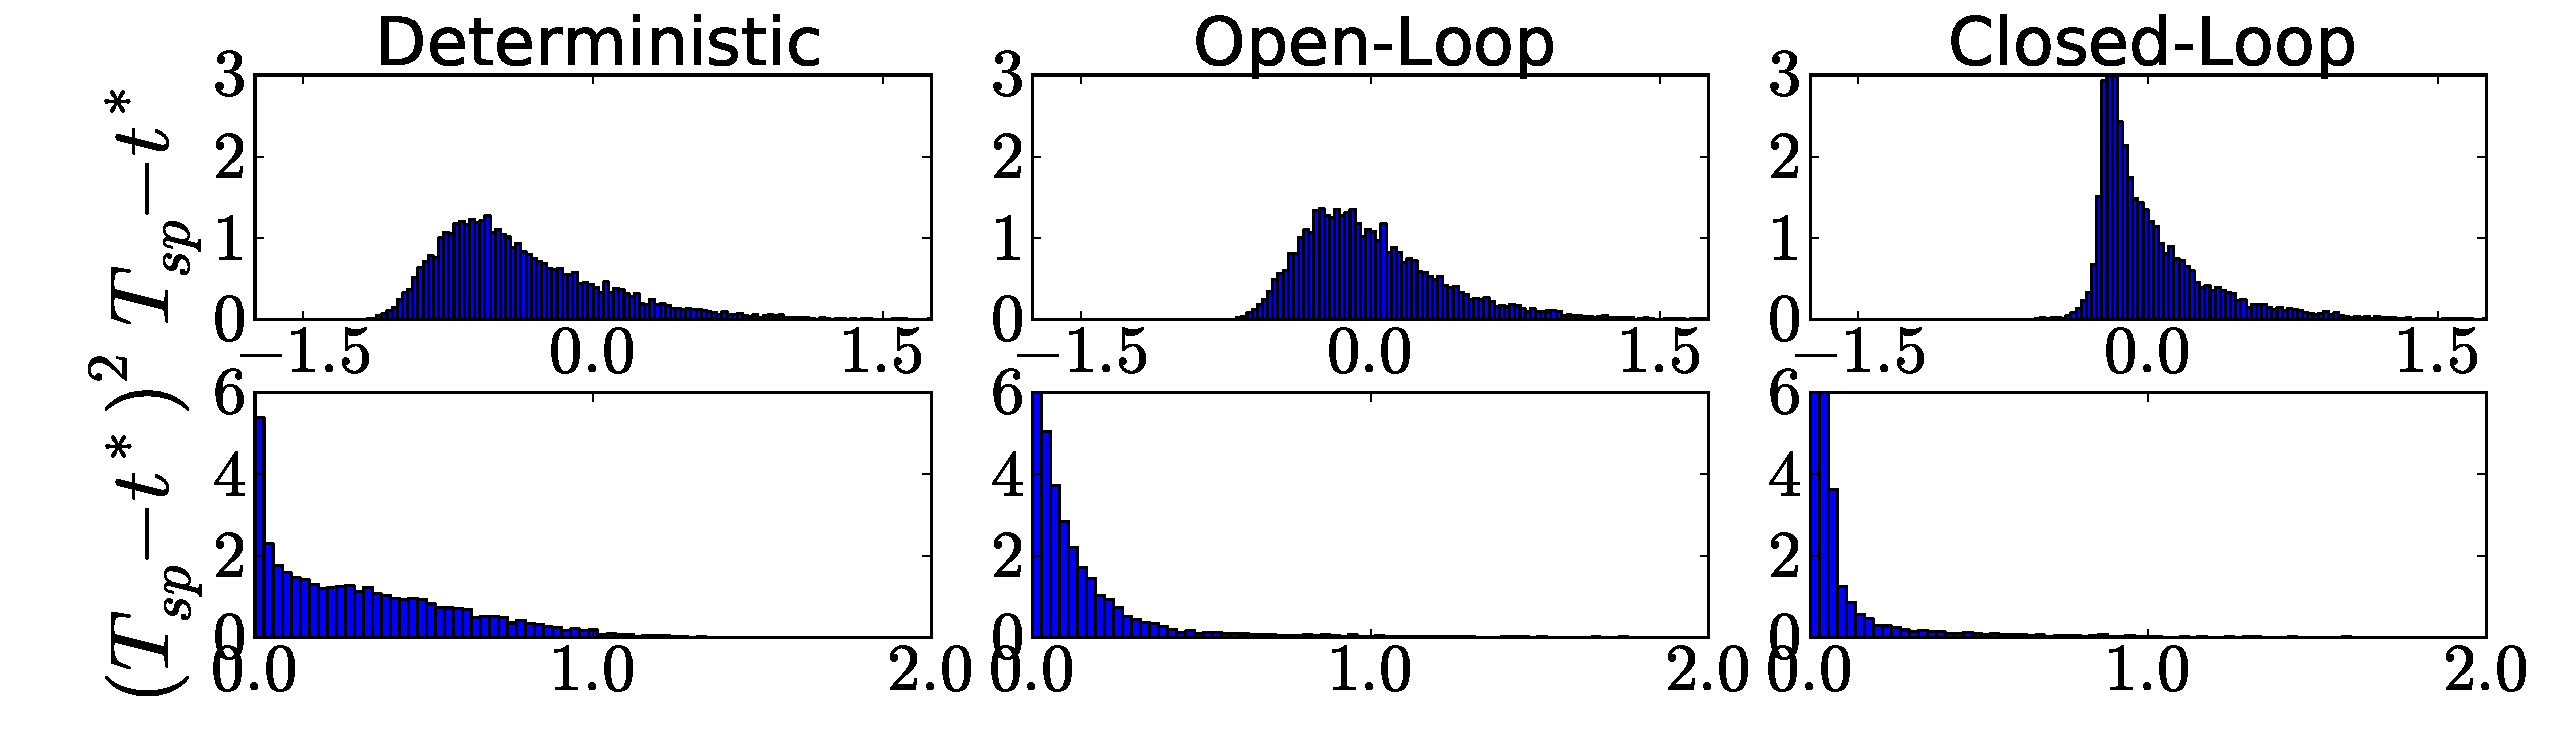
\includegraphics[width=\textwidth] 
  {Figs/ControlSimulator/Regimes_subt_ln_errors_hist.pdf} 
} 
\\ 
\subfloat[Sub-Threshold High-Noise]{ 
  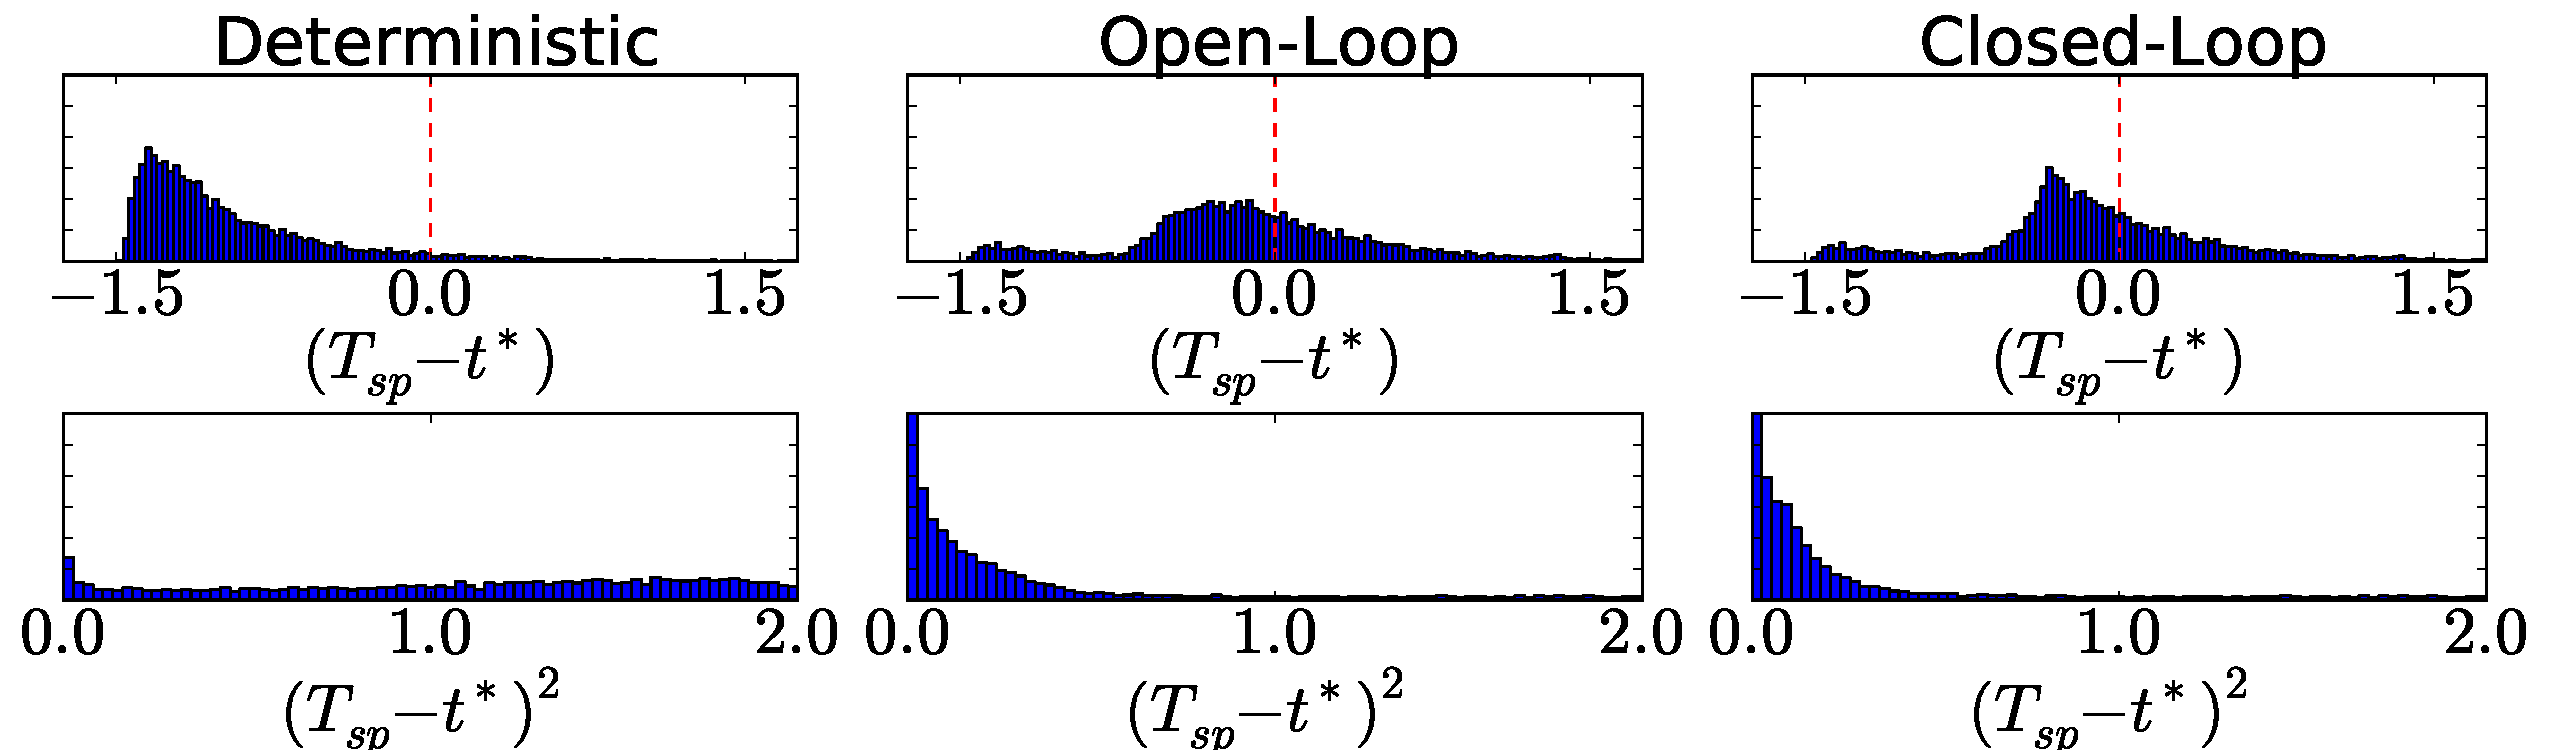
\includegraphics[width=\textwidth] 
  {Figs/ControlSimulator/Regimes_subt_HN_errors_hist.pdf} 
}\\ 
  \caption[labelInTOC]{Histogram of the spike timing error for the 
  deterministic (left) vs. open-loop stochastic (centre) vs. closed-loop 
  stochastic (right) control laws. 
  Recall that $\ts$ is the random realized spike time and $\T$ is the target 
  spike time.   
  This is for the same problem as in 
  \cref{fig:control_trajectories_examples}. 
  We have used $N=10000$ sample paths 
  to form the statistics.} 
  \label{fig:error_histograms_det_vs_openloop_vs_stoch} 
\end{center} 
\end{figure} 
\begin{figure}[h] 
\begin{center} 
\includegraphics[width=0.99\textwidth] 
{Figs/ControlSimulator/Composite_Traj.pdf}  
\caption[]{Three examples for the controlled trajectories using the 
deterministic, open-loop stochastic and closed-loop stochastic control approaches. 
The plots on the left, A,C,E, are obtained using a value of $\eps=0.001$, 
while the plots on the right, B,D,F, use $\eps=0.1$ (for a discussion on the 
effect of $\eps$ see \cref{sec:effect_of_eps}). The black vertical line in the plots indicates the 
desired spike-time, $\T$. The parameter values are $\m, \tc, \b = [0.2, 0.5,  1.5]$ (Sub-Threshold 
High-Noise regime), with $\T = 1.5$.  
The upper plots show the voltage evolution, $X(t)$, while the lower 
plots show the applied control, $\a(t)$. Note that the optimal control, $\a(t)$, obtained from 
the deterministic and from the open-loop controls are the same across all three 
samples.} 
\label{fig:control_trajectories_examples}    
\end{center}   
\end{figure} 
\begin{figure}[htp] 
\begin{center} 
  \includegraphics[width=\textwidth]{Figs/TrainController/SUPT_ln_cl_trains_sim_50.pdf} 
  \caption[ ]{How good the {\sl closed-loop} controller is at hitting a target 
  spike train. In the panel above, the blue curve is the empirical firing 
  rate of $M$ controlled trains.   strategy, the red curve is a 
  smoothed-version of the target train. (See text for details of how they are calculated). In the panel below, the 
  dashed, red lines indicate the target times, $\t_n$, while the blue dots are 
  the realizations of the controlled trains.   
  The parameters from the Super-Threshold, Low-Noise 
  regime are used. The target spike train was generated using the model itself, 
  with parameters from the Super-Threshold, High-Noise regime, without an applied 
  control, $\a=0$. 
  There are $N=16$ target spikes and $M=50$ realizations of the control strategy}  
  \label{fig:targettrain_cl_lownoise} 
\end{center} 
\end{figure}   
\begin{figure}[htp]  
\begin{center} 
  \includegraphics[width=\textwidth]{Figs/TrainController/SUPT_ln_ol_trains_sim_50.pdf} 
  \caption[ ]{How good the {\sl open-loop} controller is at hitting a target 
  spike train. 
  The drawn curves have  the same meaning as in 
  \cref{fig:targettrain_cl_lownoise}. 
  The parameters from the Super-Threshold, Low-Noise regime are used.  
  The target spike train was generated using the model itself, with parameters 
  from the Super-Threshold, High-Noise regime, without an applied control, $\a=0$. 
  There are $N=16$ target spikes and $M=50$ realizations of the control strategy} 
  \label{fig:targettrain_ol_lownoise} 
\end{center}  
\end{figure} 
\begin{figure}[htp] 
\begin{center} 
  \includegraphics[width=\textwidth]{Figs/TrainController/SUPT_HN_cl_trains_sim_50.pdf} 
  \caption[ ]{How good the {\sl closed-loop} controller is at hitting a target 
  spike train.  
  The drawn curves have  the same meaning as in 
  \cref{fig:targettrain_cl_lownoise}. 
  The parameters from the Super-Threshold, High-Noise regime 
  are used. The target spike train was generated using the model itself, with 
  parameters from the Super-Threshold, High-Noise regime, without an applied 
  control, $\a=0$. 
  There are $N=16$ target spikes and $M=50$ realizations of the control strategy} 
  \label{fig:targettrain_cl_highnoise} 
\end{center}  
\end{figure} 
\begin{figure}[htp] 
\begin{center} 
  \includegraphics[width=\textwidth]{Figs/TrainController/SUPT_HN_ol_trains_sim_50.pdf} 
  \caption[]{How good the {\sl open-loop} controller is at hitting a target 
  spike train.  
  The drawn curves have  the same meaning as in 
  \cref{fig:targettrain_cl_lownoise}. 
  The parameters from the Super-Threshold, High-Noise regime 
  are used. The target spike train was generated using the model itself, with 
  parameters from the Super-Threshold, High-Noise regime, without an applied 
  control, $\a=0$. 
  There are $N=16$ target spikes and $M=50$ realizations of the control strategy} 
  \label{fig:targettrain_ol_highnoise}     
\end{center} 
\end{figure} 
\begin{figure}[htp] 
\begin{center} 
  \includegraphics[width=\textwidth]{Figs/TrainController/SUPT_HN_cl_aplus_trains_sim_50.pdf} 
  \caption[ ]{Same as \cref{fig:targettrain_cl_highnoise}, but with the control 
  constraints, $[\amin, \amax]$ increased to $[-4,4]$ instead of $[-2,2]$.} 
  \label{fig:targettrain_cl_highnoise_aplus}     
\end{center} 
\end{figure}  
\begin{figure}[htp] 
\begin{center} 
  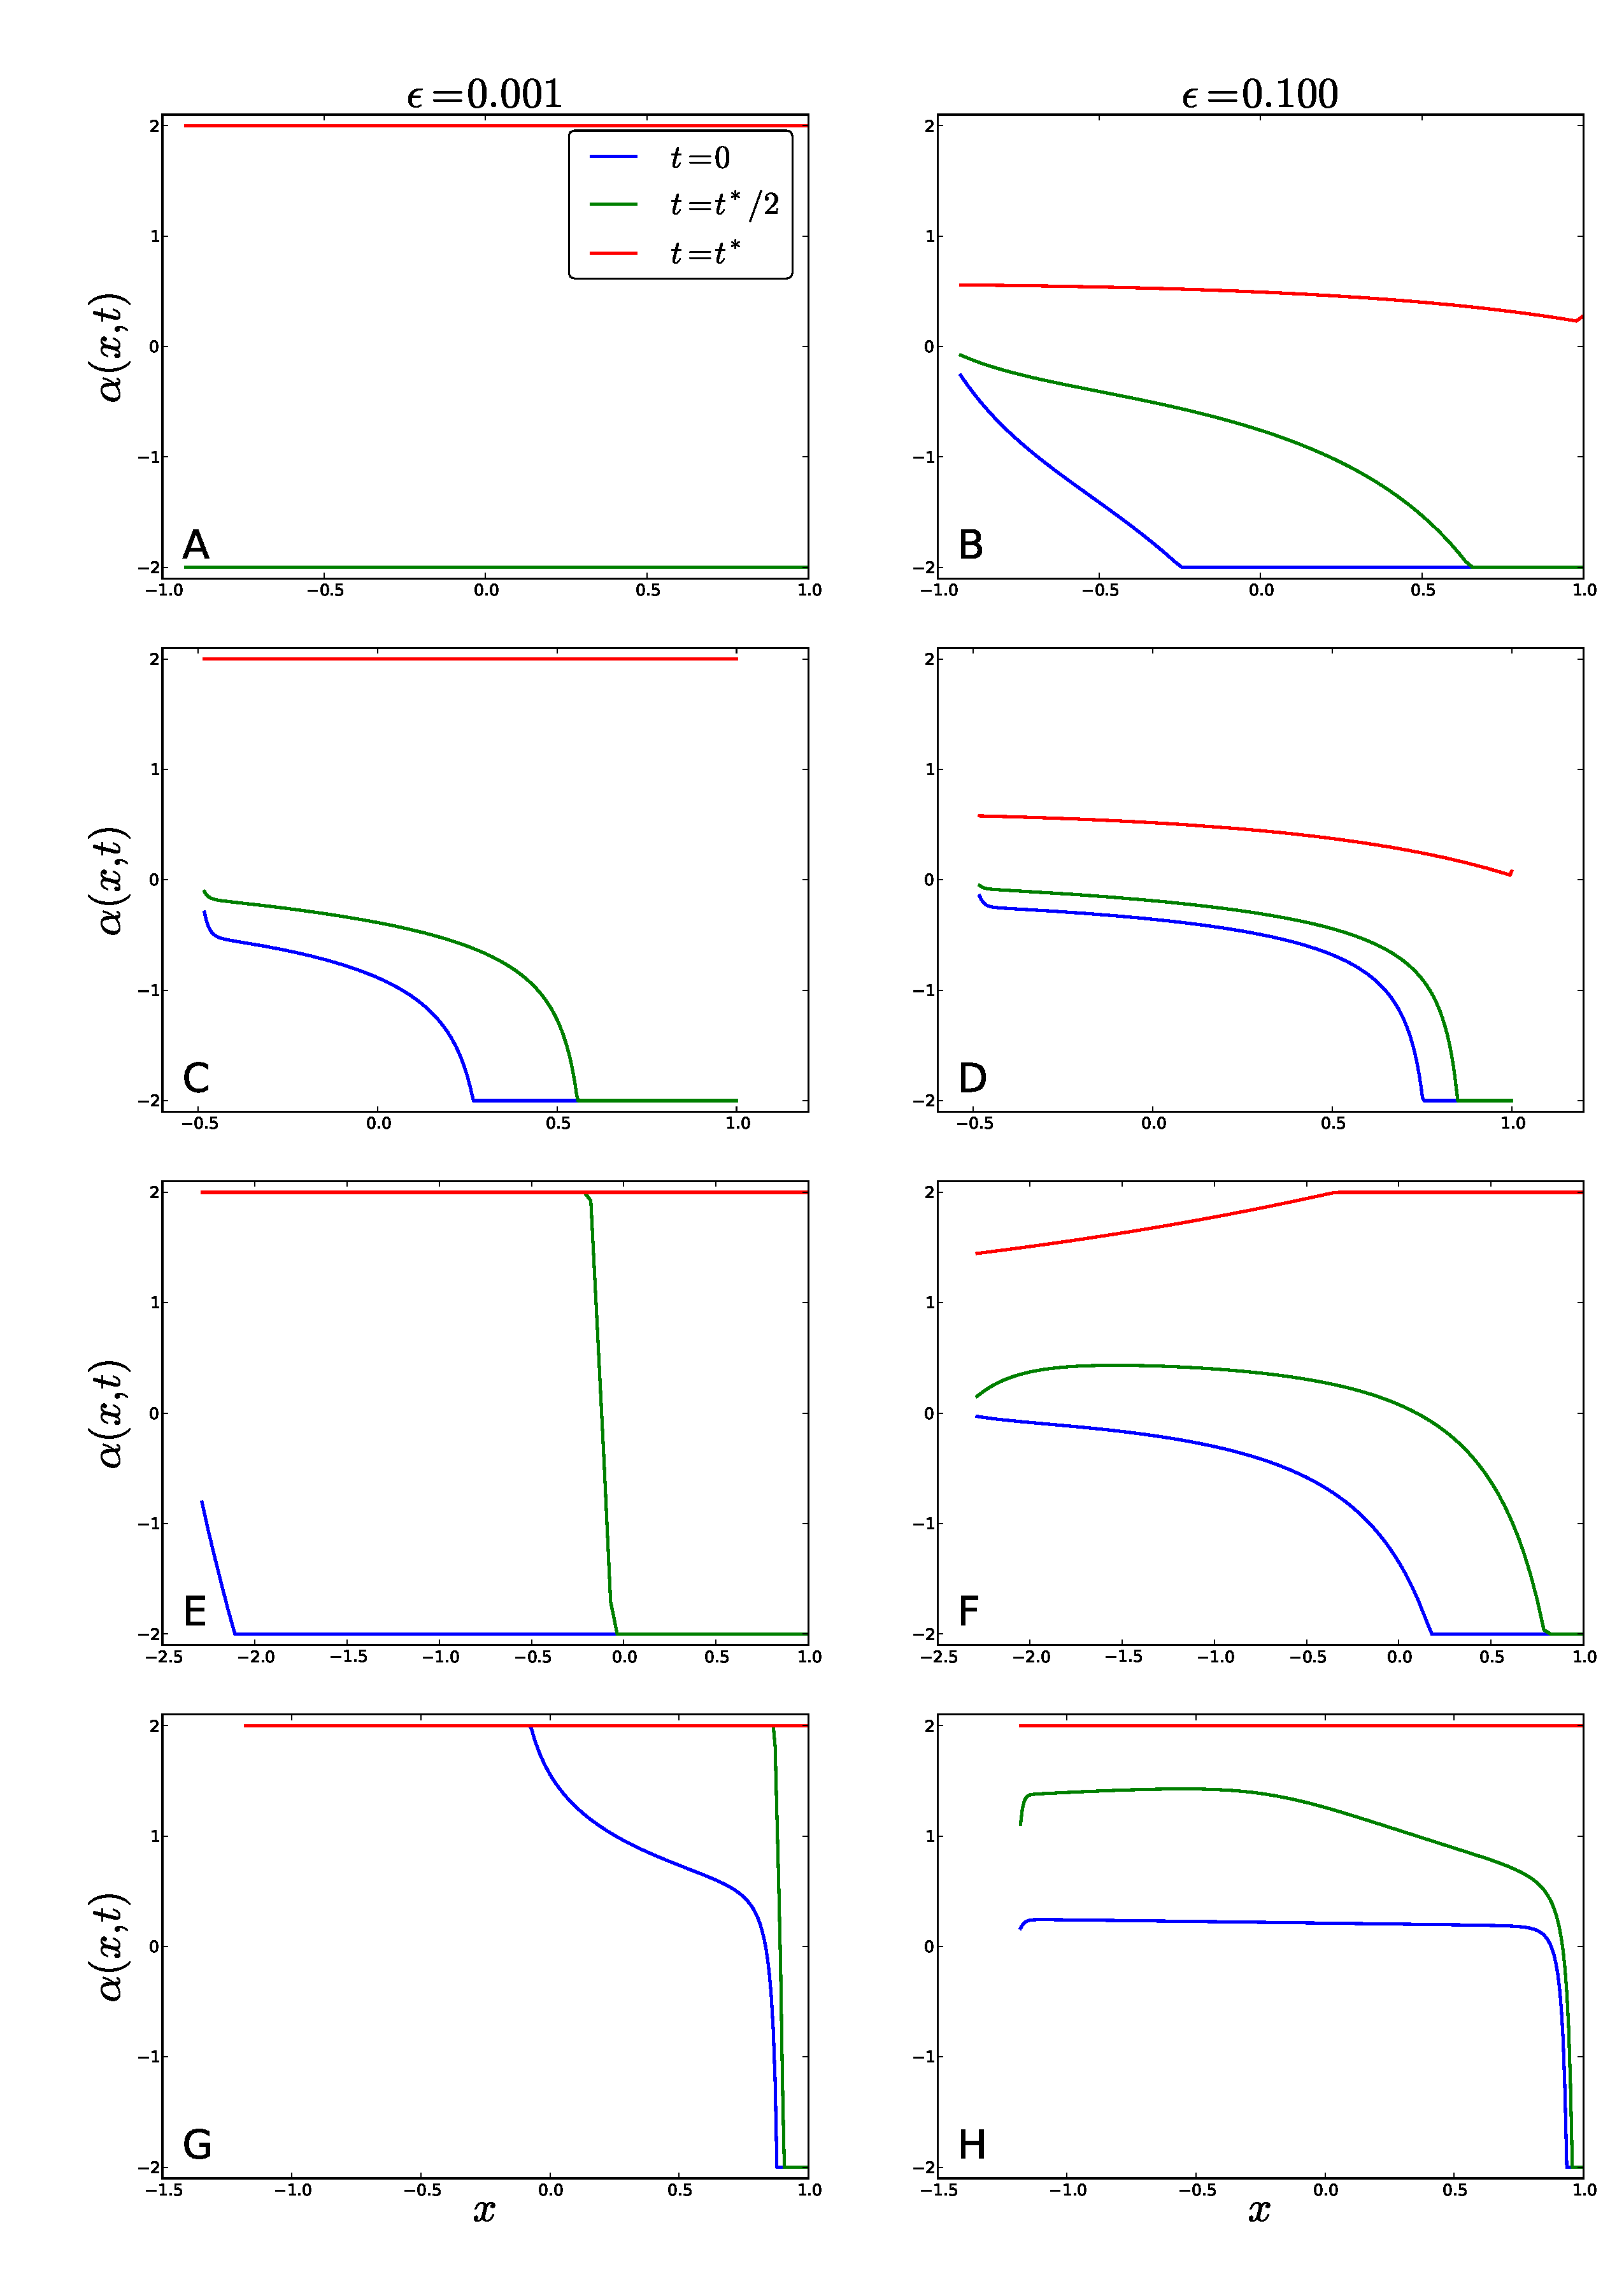
\includegraphics[width=\textwidth]{Figs/HJB/Regimes_eps_comparison.pdf} 
  \caption[labelInTOC]{Effect of $\e$ on the closed-loop control. Snapshots of 
  $\a(x,t)$ for $t$ fixed, at the start (blue), mid-point (green) and end-point 
  (red), for each of the four regimes and different values of $\eps$. 
  On the left, we use $\eps = 0.001$ and on the right $\eps = 0.1$. 
  The desired spike time is set to 
  $\T=1.5$ and the bounds are $\a \in [-2,2]$.  
  A,B) 
   Supra-Threshold-Low-Noise  
  C,D)  
   Supra-Threshold-High-Noise  
  E,F) 
   Sub-Threshold-Low-Noise  
  G,H) 
   Sub-Threshold-High-Noise} 
\label{fig:HJB_4regimes_control_different_eps}  
\end{center} 
\end{figure} 
\begin{figure}[htp] 
\begin{center} 
  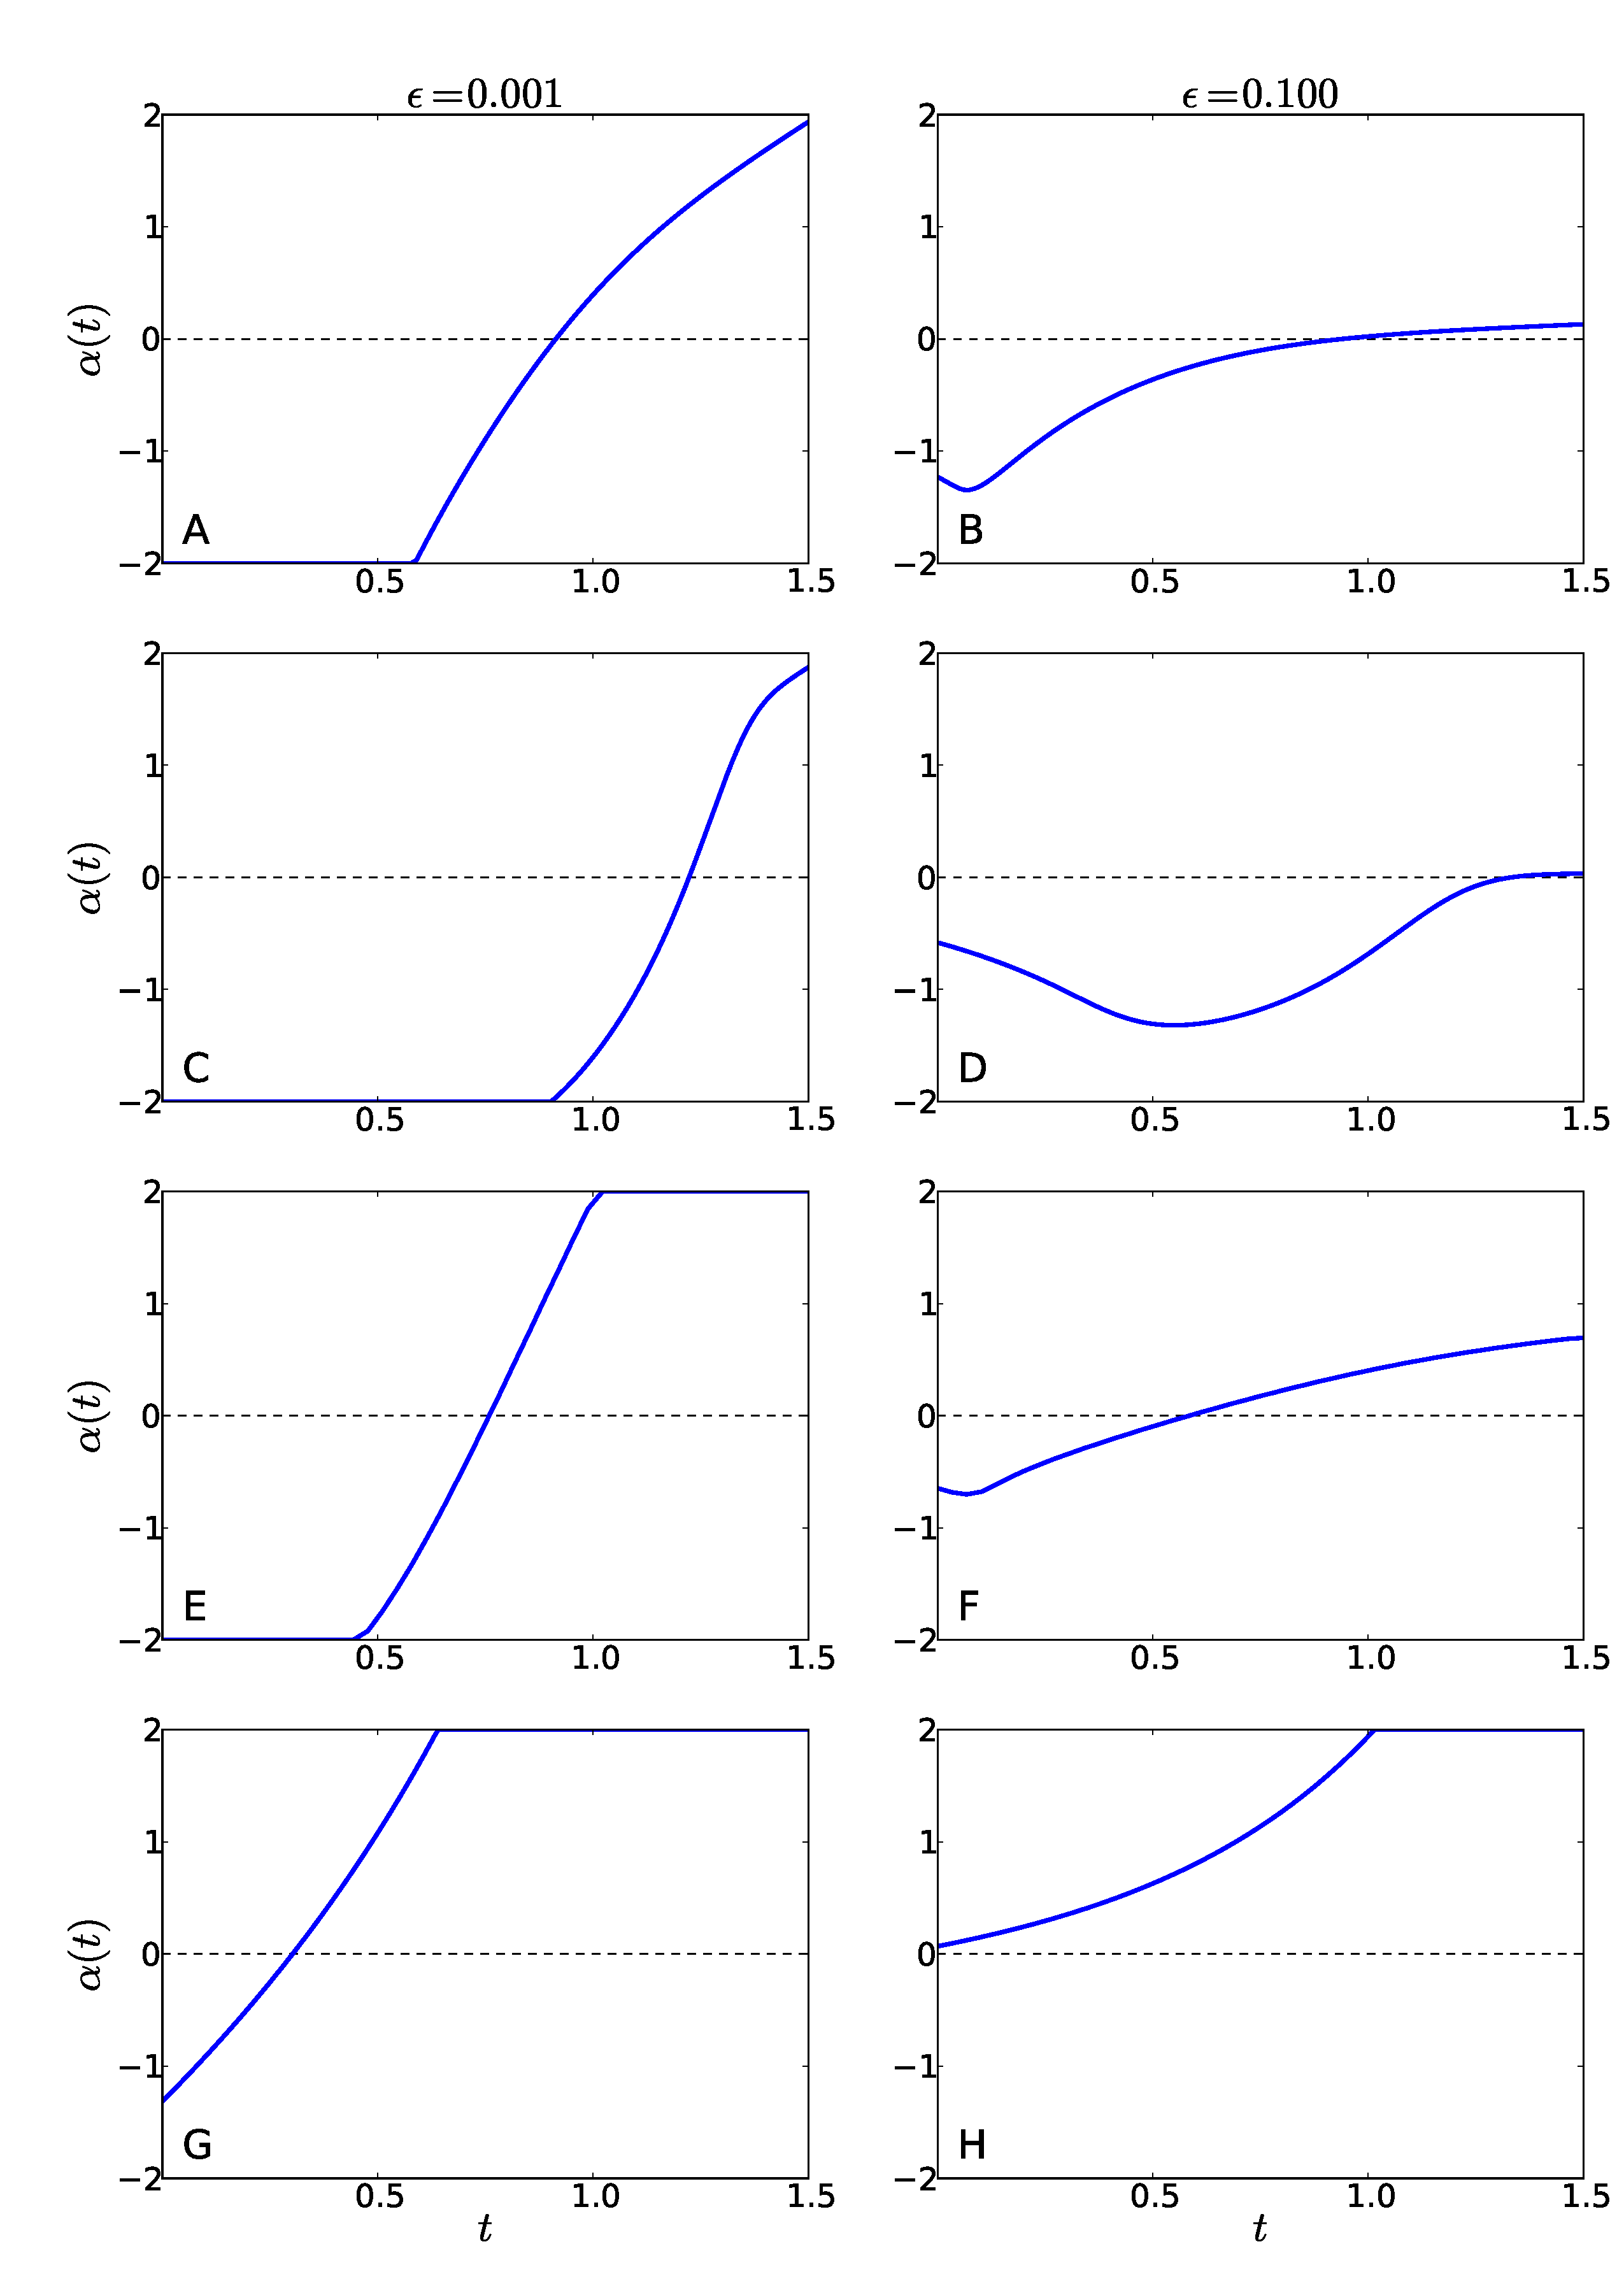
\includegraphics[width=\textwidth]{Figs/FP_Adjoint/Regimes_eps_comparison.pdf} 
  \caption[labelInTOC]{Effect of $\e$ on the open-loop control. 
  The deterministic time-trajectory of $\a(t)$ for each 
  parameter regime as function of time, $t \in [0, \T]$. 
  On the left, we use $\eps = 0.001$ and on the right $\eps =0.1$. 
  The desired spike time is set to $\T=1.5$ and the bounds are $\a \in [-2,2]$. 
    A,B) 
   Supra-Threshold-Low-Noise 
  C,D)  
   Supra-Threshold-High-Noise 
  E,F) 
   Sub-Threshold-Low-Noise 
  G,H) 
   Sub-Threshold-High-Noise} 
  \label{fig:FBK_Regimes_cs_different_es}  
\end{center} 
\end{figure} 
\clearpage
\begin{table}

\begin{tabular}{|l||{c}|{c}|}
\hline
\backslashbox{$\m$}{$\b$}
& $1.5$ & $0.3$ \\
\hline
$1.5 / \tc $ &Supra-threshold-High-noise & Supra-threshold-Low-noise \\
\hline
$0.1 / \tc$   &Sub-threshold-High-noise & Sub-threshold-Low-noise \\
\hline
\end{tabular}
\caption{Regime labels and example values. Note that for the numerical
experiments below, we use $\tc = 0.5$}
\label{tab:regimes}
\end{table}
\begin{table}[h]

\begin{center}  
\subfloat[Supra-Threshold Low-Noise]{
   \input{Figs/ControlSimulator/MeanSquaredErrors__SUPT_ln.txt}}\\ 
\subfloat[Supra-Threshold High-Noise]{   
	\input{Figs/ControlSimulator/MeanSquaredErrors__SUPT_HN.txt}}\\
 \subfloat[Sub-Threshold Low-Noise]{
 	\input{Figs/ControlSimulator/MeanSquaredErrors__subt_ln.txt}}\\ 
 \subfloat[Sub-Threshold High-Noise]{
 	\input{Figs/ControlSimulator/MeanSquaredErrors__subt_HN.txt}}\\
\caption{
Realized and theoretical performance of the different control laws. The
empirical performance is obtained using $N=10000$ sample paths. The theoretical
performance is found using the optimal value for $J$ for the open-loop
stochastic control and the value function $\v(x=0, t =0)$ for the closed-loop
stochastic control.}
\label{tab:realized_avg_errors_det_vs_openloop_vs_stoch}   
\end{center} 
\end{table} 
\begin{table}[h]

\begin{center}
 \input{Figs/ControlSimulator/Misspec_MeanSquaredErrors__subt_HN.txt}
 \caption{The effect of misspecifying the parameters. On the left, the
 system parameters and the parameters used to obtain the control are the
 same, i.e.\ correct, on the right, they are misspecified.}
\label{tab:realized_avg_errors_det_vs_openloop_vs_stoch_misspecified}
\end{center}
\end{table}

\bibliographystyle{plain}
\bibliography{library,local}

\end{document}
